\section{等式性质与不等式性质}

本节要点:
\begin{itemize}
    \item 熟练掌握等式的性质;
    \item 熟练掌握不等式的性质。
\end{itemize}

~

若$a,b,c\in \mathbb{R} $,则有等式的性质:
\begin{itemize}
    \item 性质1:$a=b\Rightarrow b=a$;
    \item 性质2:$a=b,b=c\Rightarrow a=c$;
    \item 性质3:$a=b\Rightarrow a\pm c=b\pm c$;
    \item 性质4:$a=b\Rightarrow ac=bc$;
    \item 性质5:$a=b,c\ne 0\Rightarrow a/c=b/c$。
\end{itemize}

\begin{tcolorbox}
性质1表示了对等性,性质2表示了传递性,性质3表示了加减不变性,性质4、5表示了乘除的不变性。
\end{tcolorbox}

根据算术运算的法则,不难得出不等式的性质,若$a,b,c\in \mathbb{R} $,则有不等式的性质:
\begin{itemize}
    \item 性质1:$a>b\Leftrightarrow b<a$;
    \item 性质2:$a>b,b>c\Rightarrow a>c$;
    \item 性质3:$a>b\Rightarrow a\pm c>b\pm c$;
    \item 性质4:$a>b,c>0\Rightarrow ac>bc$,$a>b,c<0\Rightarrow ac<bc$;
    \item 性质5:$a>b,c>d\Rightarrow a+c>b+d$;
    \item 性质6:$a>b>0,c>d>0\Rightarrow ac>bd$;
    \item 性质7:$a>b>0\Rightarrow a^n>b^n,n\in \mathbb{N} \text{且}n>0$。
\end{itemize}

~

等式和不等式的性质本身并无难度,关键掌握两个点。

首先,不等式在代数中表示一个约束,通常多个约束是逻辑与的关系,除非特别指明逻辑或,所以如下的三种表示方法是等价的:
\begin{align*}
&A<B,A>C \\
&C<A<B \\
&\left\{ \begin{array}{c}
	A<B\\
	A>C\\
\end{array} \right.
\end{align*}

其次,在判断两个式子的不等关系时,常用的方法是相减后和0比大小。当然也可以相除后和$\pm 1$比大小,但高中阶段不常用。

~

\begin{example}[拓广探索12,难度:$\star \star \star \star $]
火车站有某公司待运的甲种货物1530t,乙种货物1150t,现计划用A、B两种型号的货厢共50节运送这批货物。已知35t甲种货物和15t乙种货物可装满一节A型货厢,25t甲种货物和35t乙种货物可装满一节B型货厢,据此安排A、B两种货厢的节数,共有几种方案?若每节A型货厢的运费是0.5万元,每节B型货厢的运费是0.8万元,哪种方案的运费较少?
\end{example}

解:

设两种型号货厢各$A,B$个,不难得到如下4个约束:
\begin{itemize}
    \item 共运载甲种货物不少于1530t,$35A+25B\geqslant 1530$;
    \item 共运载乙种货物不少于1150t,$15A+35B\geqslant 1150$;
    \item 两种货厢共不多于50节,$A+B\leqslant 50$;
    \item 货厢为自然数,$A,B\in \mathbb{N} $。
\end{itemize}
取$A$为横坐标,$B$为从坐标,图形如下:
\begin{figure}[h]
\centering
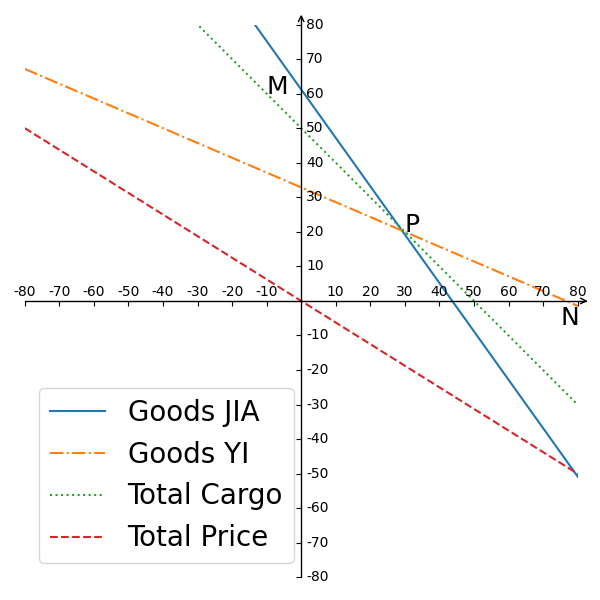
\includegraphics[height=8cm]{2.1-1.png}
\end{figure}

反映到图象上,即要求:
\begin{itemize}
    \item 共运载甲种货物不少于1530t,在蓝实线的上方;
    \item 共运载乙种货物不少于1150t,在橙点划线的上方;
    \item 两种货厢共不多于50节,在绿虚线的下方。
\end{itemize}
图中很小的一个范围。

求解:
\begin{align*}
&\because \begin{cases}
	35A+25B\geqslant 1530\\
	15A+35B\geqslant 1150\\
\end{cases} \\
&\therefore 50A+60B\geqslant 2680\Rightarrow B\geqslant \frac{2680-50A}{60} \\
&\because A+B\leqslant 50\Rightarrow B\leqslant 50-A \\
&\therefore \frac{2680-50A}{60}\leqslant 50-A \\
&\therefore A\leqslant 32
\end{align*}
$A$从32往下取自然数,的最终结果如下表:
\begin{table}[h]
\centering
\begin{tabular}{cccccc}
    \toprule
     & A型货厢 & B型货厢 & 甲种货物 & 乙种货物 & 运费\\
    \midrule
    方案一 & 30 & 20 & 1550 & 1150 & 31\\
    方案二 & 29 & 21 & 1540 & 1170 & 31.3\\
    方案三 & 28 & 22 & 1530 & 1190 & 31.6\\
    \bottomrule
\end{tabular}
\end{table}

\begin{tcolorbox}
本题很抽象,关键在于如何将生活问题转换为数学问题,即根据要求列出4个约束关系,一旦得到了这4个不等式,就完成了关键一步,余下的就是求解不等式而已。在求解不等式方面,本题只涉及一次不等式,还是很简单的。
\end{tcolorbox}




